% LaTeX source for ``การเรียนรู้ของเครื่องสำหรับเคมีควอนตัม (Machine Learning for Quantum Chemistry)''
% Copyright (c) 2022 รังสิมันต์ เกษแก้ว (Rangsiman Ketkaew).

% License: Creative Commons Attribution-NonCommercial-NoDerivatives 4.0 International (CC BY-NC-ND 4.0)
% https://creativecommons.org/licenses/by-nc-nd/4.0/

\chapter{การเลือกและปรับแต่งโมเดล}
\label{ch:reg_sel_model}

การทำให้โมเดลมีความสม่ำเสมอ (Regularization) เพื่อเพิ่มความถูกต้องและการเลือกโมเดล (Model Selection) เป็นสิ่งที่จำเป็นมากในขั้นตอน%
ของการฝึกสอนโมเดล

%--------------------------
\section{Cross Validation}
\label{sec:cross_val}
\idxen{Cross Validation}
%--------------------------

วิธีการตรวจสอบโมเดลวิธีแรกนี้เป็นวิธีที่ได้รับความนิยมเป็นอย่างมากเพราะว่าสามารถทำได้ง่ายและให้ผลลัพธ์ที่น่าเชื่อถือ นั่นก็คือ 
\enquote{K-Fold Cross Validation} หรือเรียกสั้น ๆ ว่า Cross Validation วิธีนี้เริ่มด้วยการแบ่งข้อมูล $k$ ให้มีขนาดของแต่ละส่วนเท่า ๆ กัน 
หลังจากนั้นทำเก็บข้อมูลหนึ่งส่วนไว้ใช้สำหรับเป็นตัวทดสอบโมเดลนั่นก็คือการทำ Validation แล้วทําวนไปเช่นนี้จนครบจํานวนที่แบ่งไว้ เช่น 
การทดสอบด้วยวิธี 5-fold Cross Validation ในรอบแรกเราจะทำการเทรนโมเดลด้วยชุดข้อมูลที่เกิดจากการวมส่วนที่ 2, 3, 4, และ 5 
และทำการทดสอบด้วยข้อมูลส่วนที่ 1 และในรอบที่สองเราจะเปลี่ยนมาเทรนโมเดลด้วยข้อมูลของส่วนที่ 1, 3, 4, และ 5 แล้วนำโมเดลมาทดสอบ%
ด้วยข้อมูลส่วนที่ 2

%--------------------------
\section{การคัดเลือก Feature}
\label{sec:select_feat}
\idxen{Feature Selection}
%--------------------------

การคัดเลือก Feature (Feature Selection) เป็นการหา Feature ที่เหมาะสมที่สุดสำหรับการใช้อธิบายข้อมูลของโมเลกุล โดยเราจะทำการ%
เรียงลำดับความสำคัญของ Feature แล้วทำการเลือกเฉพาะ Feature ที่คิดว่าสอดคล้องกับเอาต์พุตที่ต้องการทำนาย และคัด Feature 
ที่มีความสำคัญน้อยออกไปเพื่อหลีกเลี่ยง Bias ที่อาจจะเกิดขึ้น

%--------------------------
\section{ปัญหา Bias-Variance}
\label{sec:bias_var_prob}
\idxen{Bias-Variance}
%--------------------------

หนึ่งในปัญหาที่เราทุกคนจะต้องเจอในการสร้างโมเดลนั่นก็คือ Bias-Variance Problem ซึ่งนำไปสู่ปัญหาเรื่อง Overfitting ต่อไป
เราลองมาดูรายละเอียดกันครับ กำหนดให้โมเดลของเราแทนด้วย $\hat{f}(\vec{x})$ และค่าอ้างอิงหรือคำตอบที่เราจะมาเทียบกับการทำนายเป็น 
$y$ และความคลาดเคลื่อนที่เกิดขึ้นเป็น

\begin{equation}
    E\left[\left(y - \hat{f}(\vec{x})\right)^2\right]
\end{equation}

ซึ่งจริง ๆ แล้ว เป็นฟังก์ชันที่สมบูรณ์แบบมาก แต่ทว่าในความเป็นจริงแล้วในชุดข้อมูลของเรานั้นย่อมมี Noise $\epsilon$ ซึ่งค่าความแตกต่าง%
ระหว่างโมเดลของเรากับคำตอบก็จะมีการ Contaminate โดย $\epsilon$ ดังนี้

\begin{equation}
    y = f(\vec{x}) + \epsilon
\end{equation}

\noindent จึงทำให้ค่าความคลาดเคลื่อนที่เกิดขึ้นจริง ๆ นั้นมีสมการดังต่อไปนี้ 

\begin{align}
    E\left[\left(y - \hat{f}(\vec{x})\right)^2\right] &= 
    E\left[y^2\right] + E\left[\hat{f}(\vec{x})^2\right] - 2 E\left[y\hat{f}(\vec{x})\right] \\
    &= E\left[\left(f(\vec{x}) - \epsilon\right)^2\right] + \hat{f}(\vec{x})^2 - 2 E\left[\left(f(\vec{x}) - 
    \epsilon\right)\right]\hat{f}(\vec{x})
\end{align}

\noindent ซึ่งถ้าหากเราทำการพิสูจน์สมการด้านบนโดยพยายามจัดรูปให้อยู่ในเทอมที่มี Bias และ Variance จากชุดข้อมูล เราจะได้สมการดังต่อไปนี้

\begin{align}\label{eq:bias_variance}
E\left[\left(y - \hat{f}(\vec{x})\right)^2\right] = 
    & \underbrace{E\left[f(\vec{x}) - \hat{f}\left(\vec{x}; \mathbf{D}\right)\right]^2}_{\text{Bias}} \nonumber \\
    & + \underbrace{E\left[\left(E\left[\hat{f}\left(\vec{x}; \mathbf{D}\right)\right] - 
    \hat{f}\left(\vec{x}; \mathbf{D}\right)\right)^2\right]}_{\text{Variance}} \nonumber \\
    & + \sigma^2
\end{align}

โดยพจน์แรกนั้นจะเป็น Bias, พจน์ที่สองเป็น Variance และพจน์ที่สามเป็นค่าความแปรปรวนที่คำนวณจาก Standard Deviation ($\sigma$)
ประเด็นก็คือว่าเราสามารถควบคุม Bias กับ Variance ได้ แต่เราไม่สามารถควบคุม Noise ได้เพราะมันเป็นสิ่งที่ผูกติดมากับชุดข้อมูล ซึ่งการที่เรา%
มี Bias และ Variance ที่ไม่สมดุลกันนั้นจะทำให้เกิดผลลัพธ์ที่ตามมาในระหว่างการฝึกสอนโมเดล นั่นคือ Overfitting และ Underfitting

%--------------------------
\section{การเพิ่มประสิทธิภาพการเรียนรู้และแก้ปัญหา Overfitting}
\label{sec:fix_overfit}
%--------------------------

\begin{figure}[H]
    \centering
    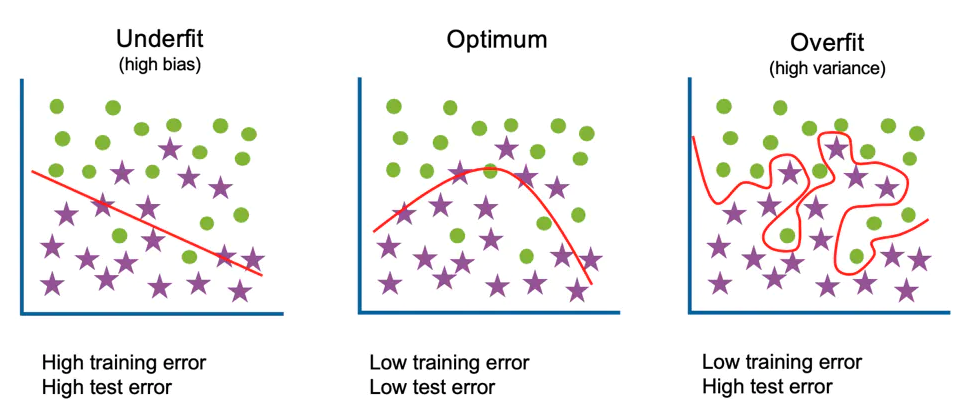
\includegraphics[width=0.9\linewidth]{fig/overfitting.png}
    \caption{โมเดลที่มีความ Overfitting และ Underfitting กับชุดข้อมูลมากเกินไป}
    \label{fig:overfitting}
\end{figure}

\begin{description}[style=nextline]
    \item[Overfitting] โมเดลตอบสนองต่อ Noise ที่มากเกินไป ทำให้เกิดการเรียนรู้และจดจำ Noise และไม่สามารถที่จะเรียนรู้รายละเอียด%
    จริง ๆ ของข้อมูลได้ ซึ่งส่งผลให้ทำนายข้อมูลไม่ได้หรือผิดพลาดมากกว่าที่คาดไว้หรือยอมรับได้ โดยกรณีนี้โมเดลจะมีค่าความแปรปรวนของข้อมูลสูง 
    (High Variance)
    
    \item[Underfitting] โมเดลของเราไม่สามารถหาความสัมพันธ์ระหว่างอินพุต ($x$) กับเอาต์พุต ($y$) ได้เพราะว่ามีข้อมูลที่ใช้ใน%
    การเทรนน้อยเกินไปหรือดึงข้อมูลออกมาจาก Training Set ได้ไม่เพียงพอที่จะเรียนรู้ โดยในกรณีนี้โมเดลจะมีค่าความเอนเอียงสูง (High Bias)

    \item[Noisy] โมเดลไม่มี Overfitting และ Underfitting แต่ยังยังมีค่า Error ของการเรียนรู้ที่ยังสูงอยู่มาก ซึ่งสาเหตุก็อาจจะมาจาก%
    การที่ชุดข้อมูล Noise มากเกินไปนั่นเอง
\end{description}

วิธีการจัดการกับ Overfitting แบบที่ง่ายที่สุดคือการเพิ่มจำนวนข้อมูลในการฝึกสอนโมเดล นอกจากนี้ยังมีวิธีอื่น ๆ ที่เราสามารถใช้ในการจัดการกับ%
ปัญหาข้างต้นได้เช่นเดียวกัน มีดังต่อไปนี้

%--------------------------
\subsection{Data Augmentation}
\label{ssec:data_aug}
\idxen{Data Augmentation}
%--------------------------

วิธีการทำ Data Augmentation นั้นจะตรงข้ามกับการทำความสะอาดข้อมูล (Data Cleaning) นั่นก็คือจะเป็นวิธีที่เราจะใส่ Noise หรือสิ่งที่%
ไม่ได้เกี่ยวข้องกับข้อมูลโดยตรงเข้าไปในชุดการฝึกสอน ก็เหมือนจะเป็นการช่วยไม่ใช่ให้เกิดการเรียนรู้ที่มันยึดติดกับชุดข้อมูลฝึกสอนมากเกินไป
วิธีการนี้ได้รับความนิยมเพราะสามารถทำได้ง่าย สะดวก และไม่มีความซับซ้อนในการทำ

%--------------------------
\subsection{Early Stopping}
\label{ssec:early_stop}
\idxen{Early Stopping}
%--------------------------

วิธี Early Stopping มีความหมายวิธีการทำงานตามชื่อเลยนั่นก็คือหยุดให้เร็วขึ้น เป็นวิธีการที่เราจะกำหนด (บังคับ) ให้การฝึกสอนหรือ Training 
นั้นหยุดก่อนที่โมเดลของเราจะเริ่มเรียนรู้ Noise ที่อยู่ภายในชุดข้อมูล แทนที่จะเรียนรู้เฉพาะชุดข้อมูลอย่างเดียว ซึ่งวิธีการนี้จะเป็นการป้องกันการเปิด 
Bias แบบตรงไปตรงมา อย่างไรก็ตามเราควรจะต้องระมัดระวังในการใช้เทคนิค Early Stopping เพราะว่าถ้าเราบังคับให้โมเดลหยุดเรียนรู้เร็วเกินไป
ปัญหาที่อาจจะเกิดขึ้นแทนการ Overfitting นั่นก็คือการ Underfitting ของโมเดล ซึ่งการเลือกจุดที่จะให้โมเดลนั้นหยุดการเรียนรู้ก็ถือว่ามีความ%
เป็น Art อย่างหนึ่ง ซึ่งจุดที่เราเลือกต้องมีความเหมาะสมระหว่าง Overfitting และ Underfitting

โค้ดของการสร้าง Callback ของ Early Stopping โดยใช้ไลบรารี่ TensorFlow 

\begin{lstlisting}[style=MyPython]
>>> callback = tf.keras.callbacks.EarlyStopping(monitor='loss', patience=3)
>>> model = tf.keras.models.Sequential([tf.keras.layers.Dense(10)])
>>> model.compile(tf.keras.optimizers.SGD(), loss='mse')
>>> history = model.fit(np.arange(100).reshape(5, 20), np.zeros(5),
...                     epochs=10, batch_size=1, callbacks=[callback],
...                     verbose=0)
>>> len(history.history['loss'])  # Only 4 epochs are run.
4
\end{lstlisting}

\noindent โดย Callback จะทำการหยุดการฝึกสอน (Training) เมื่อค่า Loss ไม่มีการลดลงภายใน 3 Epochs ที่ต่อเนื่องกัน

%--------------------------
\subsection{Ensemble Method}
\label{ssec:ensemble_model}
\idxen{Ensemble Method}
%--------------------------

เทคนิคนี้เป็นการนำโมเดลหลาย ๆ โมเดลมารวมกันเพื่อที่จะทำให้ผลลัพธ์ของการทำนายคำตอบมีค่าที่ดีที่สุด โดยโมเดล ML ที่เราจะมานำผสมกันนั้น%
จะเป็นอะไรก็ได้ เช่น Linear Regression, Logistic Regression, Gaussian Process Regression


%--------------------------
\subsection{Dropout}
\label{ssec:dropout}
\idxen{Dropout}
%--------------------------

วิธีการ Dropout เป็นเทคนิคพิเศษที่ถูกคิดค้นขึ้นมาเพื่อแก้ปัญหา Overfitting ใน Deep Learning โดยเฉพาะ ซึ่งไอเดียของเทคนิคนี้ก็คือ%
เราจะทำการตัด (Drop out หรือเอาออกไป) หน่วยการเรียนรู้ (Learning Unit หรือ Neuron) ใน Neural Network ออกไป ซึ่งจะเป็นการช่วย%
ให้โมเดลของเราลด Bias ที่เกิดจากการเรียนรู้ของข้อมูลที่มากเกินไป โดยจำนวนของ Neuron ที่จะตัดออกไปนั้นส่วนใหญ้แล้วจะคิดเป็นเปอร์เซนต์ของ
Neuron ทั้งหมด เช่น ตัดออกไป 5 เปอร์เซนต์

โค้ดของการทำ Dropout โดยใช้ไลบรารี่ TensorFlow

\begin{lstlisting}[style=MyPython]
>>> tf.random.set_seed(0)
>>> layer = tf.keras.layers.Dropout(.2, input_shape=(2,))
>>> data = np.arange(10).reshape(5, 2).astype(np.float32)
>>> print(data)
[[0. 1.]
 [2. 3.]
 [4. 5.]
 [6. 7.]
 [8. 9.]]
>>> outputs = layer(data, training=True)
>>> print(outputs)
tf.Tensor(
[[ 0.    1.25]
 [ 2.5   3.75]
 [ 5.    6.25]
 [ 7.5   8.75]
 [10.    0.  ]], shape=(5, 2), dtype=float32)
\end{lstlisting}

%--------------------------
\subsection{L1 Regularization}
\label{ssec:l1_reg}
\idxen{Regularization!L1 (LASSO)}
%--------------------------

ตามที่เราได้ศึกษาเรื่อง L1 กันไปแล้วในบทที่ \ref{ch:kernel} เราสามารถทำการปรับปรุง Loss Function ของเราได้ด้วยการเพิ่มพารามิเตอร์%
แบบพิเศษเข้าไป นั่นก็คือการใส่การลงโทษหรือ Penalty ให้กับการเรียนรู้ของโมเดล โดยการปรับพารามิเตอร์ $\lambda$ (ในบทที่ \ref{ch:kernel}
จะใช้ตัวแปร $\alpha$ ซึ่งมีความหมายเหมือนกัน) ให้เพิ่มขึ้นนั้นจะเป็นการลด Variance แต่ในขณะเดียวกันก็จะเป็นการเพิ่ม Bias โดยใน 
Linear Regression นั้นเราจะเรียก Regularization แบบ L1 ว่า LASSO

\begin{equation}
    L = \frac{1}{N}\sum_i^N \left[y_i - \hat{f}(\vec{x}_i, \vec{w}, b)\right]^2 + \lambda \sum_k \left|w_k\right|
\end{equation}

%--------------------------
\subsection{L2 Regularization}
\label{ssec:l2_reg}
\idxen{Regularization!L2 (Ridge)}
%--------------------------

สำหรับ Regularization แบบ L2 นั้นก็จะมีความคล้ายกับ L1 มาก ซึ่งวิธีนี้ในการทำ Linear Regression จะมีชื่อเรียกว่า Ridge Regression

\begin{equation}
    L = \frac{1}{N}\sum_i^N \left[y_i - \hat{f}(\vec{x}_i, \vec{w}, b)\right]^2 + \lambda \sum_k w_k^2
\end{equation}

สำหรับการเลือก Regularization นั้น ผู้เขียนขอยกประโยคของศาสตราจารย์ Frank Harrell ที่ได้แนะนำการเลือก L1 และ L2 ไว้ดังนี้
\footnote{อ้างอิง \url{https://stats.stackexchange.com/a/184022/283188}}

\blockquote{\enquote{
    Generally speaking if you want optimum prediction use L2. 
    If you want parsimony at some sacrifice of predictive discrimination use L1. 
    But note that the parsimony can be illusory, e.g., repeating the lasso process 
    using the bootstrap [introduced below] will often reveal significant instability 
    in the list of features “selected” especially when predictors are correlated with each other.
}
}
